\newpage % new page
%\stepcounter{section}
\bigskip
\phantomsection
\addcontentsline{toc}{section}{Продолжение главы 1}
\begin{center}
{\huge \bf Продолжение главы 1}\\
\end{center}
\bigskip
\gdef\SectionName{Глава \#1}
\gdef\AuthorName{ХБ}

\lhead{\ShortCourseName}
\chead{}
\rhead{\SectionName}

\cfoot{
%    \topskip0pt\vspace*{\fill}
\thepage~из~\pageref*{LastPage}
%    \vspace*{\fill}
}

\renewcommand{\headrulewidth}{0.15 mm}

\ifx\LaconicFooter\undefined
\lfoot{
%    \topskip0pt\vspace*{\fill}
Глава \#1
%    \vspace*{\fill}
}
\rfoot{
%    \topskip0pt\vspace*{\fill}
Автор: \AuthorName
%    \vspace*{\fill}
}
\renewcommand{\footrulewidth}{0.15 mm}
\fi
\Subsection{Интегральные суммы}
%BEGIN TICKET 14
\begin{definition}
    Пусть есть $[a, b]$. Тогда дробление (разбиение, пунктир) отрезка: набор точек:  $x_0 = a < x_1 < x_2 < \ldots < x_n = b$.
\end{definition}
\begin{definition}
    Ранг дробления: $\max\limits_{k=1,2,\ldots, n}(x_k - x_{k-1}) \eqqcolon |\tau|$, $\tau = (x_0, x_1, \ldots, x_n)$
\end{definition}

\begin{definition}
    Оснащение дробления --- набор точек $\xi = ( \xi_1, \xi_2, \ldots, \xi_n)$, такой что $\xi_k \in [x_{k-1}, x_k]$.
\end{definition}
\begin{definition}
    Интегральная сумма (сумма Римана) $S(f, \tau, \xi) \coloneqq = \sum\limits_{k=1}^n f(\xi_k)(x_k - x_{k-1})$, 

    \textit{По факту просто сумма площадей прямоугольников под графиком}
    \begin{figure}[h!]
    	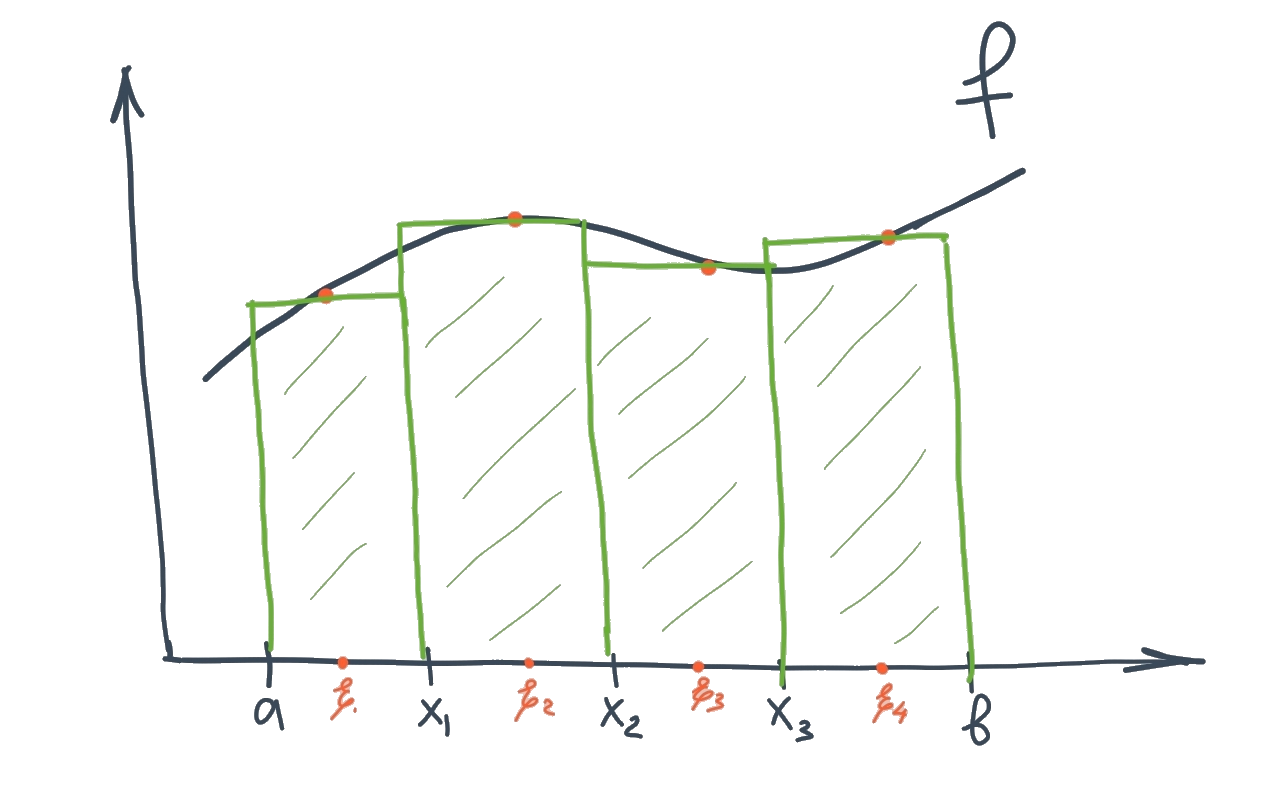
\includegraphics[scale=0.2]{riemann_sum}
    \end{figure}
\end{definition}
%END TICKET 14
%BEGIN TICKET 15
\begin{theorem}[Теорема об интегральных суммах]
    Пусть $f \in C[a, b]$,

    тогда  $|\int\limits_a^b - S(f, \tau, \xi)| \le (b-a)\omega_f(|\tau|)$.
\end{theorem}
\begin{proof}
    \[\Delta \coloneqq \int\limits_a^b f - \sum\limits_{k=1}^n f(\xi_k)(x_k - x_{k-1}) = \sum\limits_{k=1}^n \int\limits_{x_{k-1}}^{x_k} f(t)\mathrm{d}t - \sum\limits_{k=1}^n \int\limits_{x_{k-1}}^{x_k}f(\xi_k) \mathrm{d}t = \sum\limits_{k=1}^n \int\limits_{x_{k-1}}^{x_k}(f(t) - f(\xi_k))\mathrm{d}t.\] 

    \[|\Delta| \le \sum |\int \ldots| \le \sum\limits_{k=1}^n \int\limits_{x_{k-1}}^{x_k} |f(t) - f(\xi_k)| \mathrm{d}t \le \sum_{k=1}^n (x_k - x_{k-1})\omega_f(|\tau|) = (b-a)\omega_f(|\tau|).\]

    \[
        \int_{x_{k-1}}^{x_k} |f(t) - f(\xi_k)| \mathrm{d}t \le \int_{x_{k-1}}^{x_k} \omega_f(|\tau|) \mathrm{d}t = (x_k - x_{k-1}) \omega_f(|\tau|).
    .\] 
\end{proof}
\begin{consequence}
    $\forall \eps > 0 \exists \delta > 0 \forall$ дробления ранга  $\le \delta$ $\forall$ оснащения  $|\int\limits_a^b - S(f, \tau, \xi)| < \eps$
\end{consequence}
\begin{consequence}
    Если $\tau_n$~--- последовательность дроблений, ранг которых  $\to 0$, то $S(f, \tau_n, \xi_n) \to \int\limits_a^b f$.  
\end{consequence}
\begin{example}
    $S_p(n) \coloneqq 1^p + 2^p + \ldots + n^p$. Посчитаем $\lim\limits_{n \to \infty} \frac{S_p(n)}{n^{p+1}}$.

    Возьмем $f\!: [0,1] \to \R\quad f(t) = t^p$
    $\frac{S_p(n)}{n^{p+1}} = \frac{1}{n} \cdot \sum\limits_{k=1}^n \left(\frac{k}{n}\right)^p = S(f, \tau, \xi)$, где $x_k = \xi_k = \frac{k}{n}$.

    Тогда $\lim \frac{S_p(n)}{n^{p+1}} = \int\limits_0^1 t^p \mathrm{d}t = \frac{t^{p+1}}{p+1} \mid_{t=0}^{t=1} = \frac{1}{p+1}$
\end{example}

\begin{definition}
    Пусть $f\!: [a, b] \to \R$, тогда $f$  интегрируема по Риману, если $\exists I \in \R \forall \eps > 0 \exists \delta > 0 \forall$ дробления ранга  $< \delta \forall$ его оснащения  $|S(f, \tau, \xi) - I| < \eps$. 

     $I$ --- интеграл по Риману  $\int\limits_a^b f$.
\end{definition}
%END TICKET 15
%BEGIN TICKET 16
\begin{lemma}
    $f \in C^2[\alpha, \beta]$. Тогда  \[\int\limits_\alpha^\beta f(t)\mathrm{d}t - \frac{f(\alpha) + f(\beta)}{2}(\beta - \alpha) = -\frac{1}{2} \int\limits_\alpha^\beta f''(t)(t-\alpha)(\beta-t)\mathrm{d}t.\]
\end{lemma}
\begin{proof}
    Пусть  $\gamma \coloneqq \frac{\alpha + \beta}{2}$. Тогда: \[
        \int\limits_\alpha^\beta f(t) \mathrm{d}t = \int\limits_\alpha^\beta f(t)(t-\gamma)' \mathrm{dt} = f(t)(t-\gamma)\mid_{t=\alpha}^{t=\beta} - \int\limits_\alpha^\beta f'(t)(t-\gamma)\mathrm{dt}
    .\] 
    Заметим, что $f(t)(t-\gamma)\mid_{t=\alpha}^{t=\beta} = f(\beta)(\beta - \gamma) - f(\alpha)(\alpha - \gamma) = \frac{f(\alpha) + f(\beta)}{2}(\beta - \alpha)$. Продолжим: \begin{align*}
        \text{левая часть} &= -\int_{\alpha}^\beta f'(t)(t-\gamma)\mathrm{d}t = \frac{1}{2}\int_\alpha^\beta f'(t)((t-\alpha)(\beta-t))' \mathrm{d}t = \\ &= \frac{1}{2}f'(t)(t-\alpha)(\beta - t)\mid_{t=\alpha}^{t=\beta} - \frac{1}{2} \int_\alpha^\beta f''(t)(t-\alpha)(\beta-t)\mathrm{d}t
    .\end{align*}

    Переход к $((t-\alpha)(\beta - t))'$: \[
        ((t-\alpha)(\beta - t))' = (-t^2 + (\alpha + \beta)t - \alpha\beta)' = -2t+(\alpha + \beta) = -2(t-\gamma)
    .\] 
\end{proof}
\begin{remark}
    $\frac{f(\alpha) + f(\beta)}{2}(\beta - \alpha)$~--- площадь трапеции:
    \begin{figure}[h!]
    	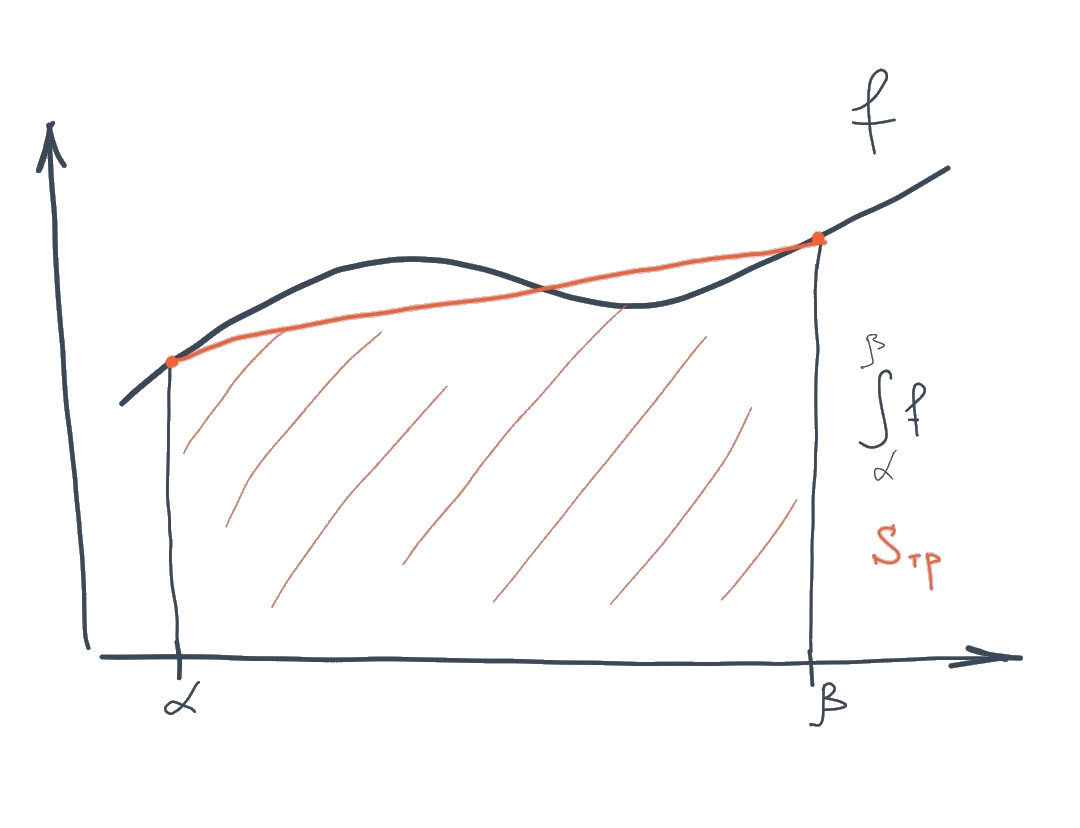
\includegraphics[scale=0.16]{riemann_trapezoid}
    \end{figure}
\end{remark}

\begin{theorem}[Оценка погрешности в формуле трапеции]
    Пусть $f \in C^2[a, b]$.

    Тогда : \[\left|\int\limits_a^b f(t) \mathrm{d}t - \sum_{k=1}^n \frac{f(x_{k-1}) + f(x_k)}{2}(x_k - x_{k-1})\right| \le \frac{|\tau|^2}{8} \int\limits_a^b |f''|\]
\end{theorem}
\begin{proof}
    $\Delta \coloneqq \int\limits_a^b - \sum \ldots = \sum\limits_{k=1}^n \int\limits_{x_{k-1}}^{x_k}f(t)\mathrm{d}t - \sum\limits_{k=1}^n \frac{f(x_{k-1}) + f(x_k)}{2}(x_k - x_{k-1})$

    \begin{align}
        |\Delta| \le  \sum\limits_{k=1}^n |\int\limits_{x_{k-1}}^{x_k} f(t)\mathrm{d}t - \frac{f(x_{k-1}) + f(x_k)}{2}(x_k - x_{k-1})| = \frac{1}{2} \sum\limits_{k=1}^n \left| \int_{x_{k-1}}^{x_k} f''(t)(t-x_{k-1})(x_k - t)\mathrm{d}t\right|
    .\end{align} Тогда вспомним, что $(t-x_{k-1})(x_k - t) \le \left( \frac{x_k - x_{k-1}}{2}\right)^2 \le \frac{|\tau|^2}{4} \implies (4) \le \frac{1}{2} \sum\limits_{k=1}^n\ \int\limits_{x_{k-1}}^{x_k}|f''(t)| \cdot \frac{|\tau|^2}{4} \mathrm{d}t = \frac{|\tau|^2}{8} \sum \int\limits_{x_{k-1}}^{x_k} |f''| = \frac{|\tau|^2}{8} \cdot \int\limits_a^b |f''|$
\end{proof}
\begin{remark}
    Пусть разбиение на $n$ равных отрезков  $x_k - x_{k-1} = \frac{b-a}{n} = |\tau|$:
    \[
        \sum_{k=1}^n \frac{f(x_{k-1}) + f(x_k)}{2}(x_k - x_{k-1}) = \frac{b-a}{n} \sum_{k=1}^n \frac{f(x_{k-1}) + f(x_k)}{2} = \frac{b-a}{n}(\frac{f(x_0)}{2} + \sum_{k=1}^{n-1}f(x_k) + \frac{f(x_n)}{2})
    .\] 
\end{remark}
\begin{remark}
    Возьмем разбиение на равные отрезки и $\xi_k = x_k$:
     \[
         S(f, \tau, \xi) = \sum_{k=1}^n f(\xi_k)(x_k - x_{k-1}) = \frac{b-a}{n} \sum_{k=1}^n f(x_k)
    .\] 
\end{remark}
%END TICKET 16
%BEGIN TICKET 17
\begin{theorem}[формула Эйлера-Маклорена]
    Пусть $f \in C^2[m, n]$, тогда
     \[
         \sum_{k=m}^n f(k) = \frac{f(m) + f(n)}{2} + \int_m^n f(t) \mathrm{d}t + \frac{1}{2} \int_m^n f''(t)\{t\}(1-\{t\})\mathrm{d}t
    .\]
\end{theorem}
\begin{proof}
    Подставим $\alpha = k$ и  $\beta = k + 1$ в лемму:
    \begin{align*}
        \int_{k}^{k+1} f(t) \mathrm{d}t &= \frac{f(k) + f(k + 1)}{2} - \frac{1}{2} \int_k^{k+1} f''(t)(t-k)(k+1-t) \mathrm{d}t = \\ &= \frac{f(k) + f(k + 1)}{2} - \frac{1}{2} \int_{k}^{k+1} f''(t) \{t\}(1-\{t\}) \mathrm{d}t
        .\end{align*} Дальше суммируем по $k$ от  $m$ до  $n-1$:  \[
    \int_m^n f(t) \mathrm{d}t = \sum_{k=m}^{n-1} \frac{f(k) + f(k + 1)}{2} - \frac{1}{2} \int_m^n f''(t)\{t\}(1-\{t\}) \mathrm{d}t
.\] Заметим, что $\sum\limits_{k=m}^{n-1} \frac{f(k) + f(k + 1)}{2} = \frac{f(m) + f(n)}{2} + \sum_{k=m+1}^{n-1} f(k)$. И тогда: 
\[
    \sum_{k=m}^n f(k) = \frac{f(m) + f(n)}{2} + \int_m^n f(t)\mathrm{d}t + \frac{1}{2} \int_m^n f''(t)\{t\}(1-\{t\})\mathrm{d}t
.\] 
\end{proof}
%END TICKET 17
%BEGIN TICKET 18
\begin{example}
    $S_p(n) = 1^p + 2^p + \ldots + n^p$, $f(t) = t^p$,  $m = 1$,  $f''(t) = p(p-1)t^{p-2}$.

    $S_p(n) = \frac{1+n^p}{2} + \int\limits_1^n t^p \mathrm{d}t + \frac{1}{2} \int\limits_1^n p(p-1)t^{p-2} \{t\}(1-\{t\}) \mathrm{d}t$.

    При $p \in (-1, 1)$  $\int_1^n t^p \mathrm{d}t = \frac{t^{p+1}}{p+1} \mid_1^n = \frac{n^{p+1}}{p+1} - \frac{1}{p+1} = \frac{n^{p+1}}{p+1} + \mathcal{O}(1)$.\[
        \int_1^n t^{p-2} \underbrace{\{t\}(1-\{t\})}_{\le \frac{1}{4}} \mathrm{dt} \le \frac{1}{4} \int_1^n t^{p-2} \mathrm{d}t = \frac{1}{4} \cdot \frac{t^{p-1}}{p-1} \mid_1^n = \frac{1}{4} \cdot \frac{n^{p-1} - 1}{p - 1} = \mathcal{O}(1)
    .\] 

    То есть $S_p(n) = \frac{n^{p+1}}{p+1} + \frac{n^p}{2} + \mathcal{O}(1)$.

    При $p > 1$  $S_p(n) = \frac{n^{p+1}}{p+1} + \frac{n^p}{2} + \mathcal{O}(n^{p-1})$.
\end{example}
\begin{example}
    Гармонические числа: $H_n \coloneqq 1 + \frac{1}{2} + \frac{1}{3} + \ldots + \frac{1}{n}$. $m = 1, f(t) = \frac{1}{t}, f''(t) = \frac{2}{t^3}$.
    \[
    H_n = \frac{1 + \frac{1}{n}}{2} + \int_1^n \frac{\mathrm{d}t}{t} + \frac{1}{2} \int_1^n \frac{2}{t^3}\{t\}(1-\{t\})\mathrm{d}t
    \] Откуда получаем ($a_n \coloneqq \int\limits_1^n \frac{\{t\}(1-\{t\})}{t^3}$; $\int_1^n \frac{\mathrm{d}t}{t} = \ln t \mid_1^n = \ln n$): \[
H_n = \ln n + \frac{1}{2} + \frac{1}{2n} + a_n
.\] Заметим, что $a_{n+1} = a_n + \int\limits_n^{n+1}\frac{\{t\}(1-\{t\})}{t^3} \mathrm{d}t > a_n$. То есть $a_n\uparrow$. Причем $a_n \le \int\limits_1^n \frac{\mathrm{d}t}{t^3} = -\frac{1}{2t^2} \mid_1^n = \frac{1}{2} - \frac{1}{2n^2} < \frac{1}{2}$. А значит $a_n$ имеет предел, а значит  $a_n = a + o(1)$.
\\
Вывод:  $H_n = \ln n + \gamma + o(1)$, где  $\gamma \approx 0.5772156649$ --- постоянная Эйлера.
\end{example}
\begin{remark}
    $H_n = \ln n + \gamma + \frac{1}{2n} + \mathcal{O}(\frac{1}{n^2})$~--- точная формула.
\end{remark}
%END TICKET 18
%BEGIN TICKET 19
\begin{example}[Формула Стирлинга]
    $m = 1, f(t) = \ln t, f''(t) = -\frac{1}{t^2}$.

    \[
        \ln n! = \sum_{k=1}^n \ln k = \underbrace{\frac{\ln 1 + \ln n}{2}}_{= \frac{1}{2} \ln n} + \underbrace{\int_1^n \ln t \mathrm{d}t}_{\mathclap{=t\ln t-t\mid_1^n = n\ln n - n + 1}} - \underbrace{\frac{1}{2} \int_1^n \frac{\{t\}(1-\{t\})}{t^2} \mathrm{d}t}_{\coloneqq b_n} \Rightarrow \ln n! = \frac{1}{2} \ln n + n \ln n - n + 1 - b_n
    .\] 
    Посмотрим на $b_n$:  \[
        b_n \le \frac{1}{2} \int_1^n \frac{\mathrm{d}t}{t^2} = \frac{1}{2} (-\frac{1}{t}) \mid_1^n = \frac{1}{2} (1-\frac{1}{n}) < \frac{1}{2} \implies b_n = \underbrace{b}_{=\lim b_n} + o(1)
    .\] 

    А значит $\ln n! = n \ln n - n + \frac{1}{2} \ln n + (1-b) + o(1)$. \\
    Можем найти $b$, для этого представим обе части как экспоненты: $n! = n^n e^{-n} \sqrt{n} e^{1-b} e^{o(1)} \sim n^n e^{-n} \sqrt{n} C$.

    Вспомним (из следствия формулы Валлиса): $\binom{2n}{n} \sim \frac{4^n}{\sqrt{\pi n}}$. А еще знаем, что $\binom{2n}{n} = \frac{(2n)!}{(n!)^2} \sim \frac{(2n)^{2n}e^{-2n}\sqrt{2n}C}{(n^n e^{-n}\sqrt{n}C)^2} = \frac{4^n \sqrt{2}}{\sqrt{n}C}$.

    Тогда получаем, что $\frac{4^n}{\sqrt{\pi n}} \sim \frac{4^n \sqrt{2}}{\sqrt{n}C} \implies C \sim \frac{4^n \sqrt{2}}{\sqrt{n}} \cdot \frac{\sqrt{\pi n}}{4^n} = \sqrt{2\pi}$.

    Итоговый результат (Формула Стирлинга): \begin{align*}
        n! &\sim n^n e^{-n} \sqrt{2\pi n}\\
        \ln n! &= n \ln n - n + \frac{1}{2} \ln (2\pi n) + o(1)
    .\end{align*}
\end{example}
\begin{remark}
    Если посчитать точнее, то получим $\ln n! = n \ln n - n + \frac{1}{2} \ln(2 \pi n) + \mathcal{O}(\frac{1}{n})$.
\end{remark}
%END TICKET 19
